\documentclass[a4paper]{article}

\usepackage[utf8]{inputenc}
\usepackage[portuges]{babel}
\usepackage{a4wide}
\usepackage{multicol}
\usepackage{spverbatim}
\usepackage{graphicx}

\title{Projeto de LI1 - Sokoban\\Grupo 163}
\author{Sérgio Jorge (A77730) \and José Martins (A78821)}

\begin{document}

\maketitle

\begin{abstract}
Neste relatório vamos fazer uma análise acerca do trabalho realizado na segunda fase do projecto no âmbito da UC de Laboratórios de Informática I com o objetivo de desenvolver o jogo Sokoban na linguagem Haskell, com recurso à biblioteca Gloss. Contudo, o relatório apresenta também o jogo realizado pelo nosso grupo com ajuda das várias tarefas resolvidas propostas pelas professores de modo a facilitar o desenvolvimento do mesmo bem como, todo o processo do mesmo.
\end{abstract}

\tableofcontents

\section{Introdução}
\label{sec:intro}

Este projeto foi realizado com o objetivo de construir um jogo, o Sokoban, semelhante ao apresentado em sokoban.info. Foram propostas pelos professores, 6 tarefas computacionais, realizadas na linguagem Haskell, na qual a conclusão e a interligação de 5 delas permitiu a realização da última, o desenvolvimento do jogo. As 5 tarefas permitiu por um lado, melhorar e consolidar os conhecimentos da linguagem, visto que para resolver as tarefas foi necessário recorrer à documentação e a conhecimentos lecionados na UC de Programação Funcional. Por outro, permitiu aprender processos na resolução de problemas, porque solucionou-se pequenos problemas simples de modo a concluir cada tarefa sendo que a resolução das tarefas ajudou a desenvolver o objetivo e problema principal, daí o provérbio "Dividir para reinar". Como a maior parte do trabalho já estava feito na altura da realização do jogo, devido ao facto anteriormente apresentado, apenas faltou adicionar certos extras de forma a tornar o jogo mais completo e belo. Assim, de modo a facilitar a compreensão do projeto, o relatório está dividido da seguinte maneira:
\begin{description}
    \item[Secção 2 :] Apresentação do problema;
    \item[Secção 3 :] Resolução do problema;
    \item[Secção 4 :] Conclusões do projeto.
\end{description}

\section{Problema}
\label{sec:problema}

Na segunda fase do projeto de LI1, subordinado ao jogo Sokoban, é-nos pedido para dar continuidade ao trabalho realizado na primeira fase do projeto, onde tínhamos como objetivo, validar um mapa dado, visualizar o mapa e calcular o estado resultado da execução de um comando. A 2º tarefa da 1º fase do projeto (visualizar o mapa) ajuda também na produção do jogo visto que facilita desenhar o mapa no ecrã bem como para saber se o jogo já finalizou ou não.
Mas, a 2º fase é a que permitirá, de certa forma, encadear da melhor maneira todos os processos necessários para o jogo correr. Assim, foram definidas tarefas (tal como na fase 1) a realizar.
\begin{description}
\item[Tarefa D]\hfill \\ 
O código deverá ser capaz de calcular o resultado de toda a execução de uma sequência de comandos dada na última linha do input e deverá fazê-lo até ao fim do puzzle ou até ao fim do último comando. Esta é uma parte que ainda não envolve ambiente gráfico e deve apresentar, como output, uma linha com o texto "FIM" ou "INCOMPLETO" assim como, o número de comandos executados. Há ainda a dizer que o texto depende da configuração final que for atingida.

A tarefa serve como uma base para a implementação de eventos, ou seja, o programa deverá, depois, ser capaz de saber como reagir a determinados comandos do teclado do utilizador e como estes influenciam e são influenciados pelo jogo.
\item[Tarefa E]\hfill \\ 
Nesta parte do projeto, é suposto determinar-se a largura e a altura do menor retângulo que consiga envolver uma Picture da biblioteca Gloss. 

É um exercício que tem por finalidade, fazer com que haja e surja um conhecimento considerável em relação à biblioteca em questão.
\item[Tarefa F]\hfill \\
Esta é a tarefa em que se concretiza o próprio jogo \emph{Sokoban} englobando e juntando a parte de código com a parte gráfica. O objetivo é proporcionar ao utilizador um jogo numa janela gráfica, com a qual se torna possível interação e na qual devem estar implementadas todas as regras e funcionalidades fieis ao jogo original \emph{Sokoban}.

\end{description}

\section{Solução}
\label{sec:solucao}

\subsection{Estruturas de Dados}

As estruturas de dados são bastante importantes no desenvolvimento do jogo pois permite a transformação e armazenamento dos dados. Destaca-se neste trabalho as seguintes estruturas:

\begin{description}
    \item[String/lista de String :] Essenciais ao longo de todo o projeto pois contém os mapas;
    \item[lista de (Int,Int) :] Usado no armazenamento de coordenadas;
    \item[Picture :] Permite desenhar a parte gráfica do jogo;
    \item[Command :] Essencial para a mudança das coordenadas do boneco e das caixas;
    \item[Events :] Inputs do teclado, do rato, etc. Essencial no jogo, pois após um input altera-se o estado geral do jogo (Seja mover o boneco, seja alterar de nivel, etc);
    \item[Mapa :] Principal tipo no jogo, pois possui a informação 'instantânea' essencial para alterar o estado geral do jogo, ou seja com este tipo podemos alterar quase tudo no jogo.
\end{description}

\subsection{Implementação}
\subsubsection{Tarefa D}
Já que nesta parte é necessário calcular o resultado de toda a execução de uma sequência de comandos dada na última linha do input, é evidente que é recebido um mapa válido com comandos como "U","L","R" e "D" que estão relacionados com o caminho que a personagem deve assumir no jogo em si. 

Então, para começar, é preciso tratar os dados do input e, portanto, faz-se a divisão em tabuleiro e coordenadas através da função parteMapaB que, usa SplitAt com auxílio da função contaListasMapa para saber quando é que tem de fazer a divisão.
Depois, com a função colocaCaixas e depois de lidas as coordenadas das caixas do input, colocamos-as no mapa.

Com o mapa preparado, é então altura de colocarmos o boneco a mover-se. Relativamente às coordenadas da personagem, são também usadas duas funções: sTOI que converte uma string numa lista de dois números e liTOT que recebe uma lista de dois números e converte num tuplo. Depois, temos a função mudaCoordsCaixas que muda as coordenadas das caixas caso o boneco empurre uma delas. É também importante evidenciar a presença da função verificaMov que verifica se o movimento é válido. Relativamente aos comandos, a função converteC converte o carater para Command e converteString que converte uma string de comandos numa lista de Command.
Há também a contagem do número de comandos executados que é necessária para o output da tarefa.

Assim, a tarefa tem por base uma condição que devolve "FIM" ou "INCOMPLETO" tendo em conta a veracidade da função verificaCI. Esta é uma função que trata de verificar se dadas aquelas coordenadas de caixas e da personagem e dados aqueles comandos, é possível ou não completar o puzzle.

\subsubsection{Tarefa E}
Para a resolução desta tarefa e dado que os construtores ThickCircle, Arc, ThickArc e Text não podem ser envolvidos num retângulo, centrámos as nossas atenções nos construtores Polygon, Line, Circle, Bitmap, Color, Translate, Rotate, Scale e Pictures.
Antes de mais, construímos a função larAlt (que serve como a base da tarefa) que dada uma Path converte num tuplo de Floats e o que essa função faz é primeiro aplicar unzip.

\begin{verbatim}
unzip :: [(a, b)] -> ([a], [b])
\end{verbatim}

Depois faz-se a subtração entre o máximo de a e o mínimo de a e a subtração entre o máximo de b e o mínimo de b. Com isto, e dado que uma Path é uma lista de pontos, conseguimos saber a distância entre os pontos mais distantes, ou como quem diz, a largura e a altura. Assim, com esta função, temos como objetivo converter tudo para Path porque daqui podemos tirar a largura e a altura.
Em relação aos diferentes construtores:

\begin{description}
  \item[Polygon e Line :] dado que o argumento de polygon e da line é um Path, a largura e a altura do retângulo é dada pela aplicação da função larAlt aos construtores;
  \item[Circle :] dado um certo raio calculamos vários pontos da circunferência segundo uma função matemática resultando disso um conjunto de pontos;
  \item[Bitmap :] a partir da altura e largura dada pelo construtor Bitmap calculamos os quatro pontos extremos do retangulo da imagem;
  \item[Color :] como a função Color em nada altera o conjunto de pontos e consequentemente a largura e a altura, então ignoramos a função;
  \item[Translate :] usamos uma função auxiliar (translateM) que recebe dois argumentos (x e y) e um conjunto de pontos (Path) e soma o argumento x aos 1º elementos do conjunto dos pontos e o argumento y aos 2º elementos do conjunto de pontos de forma a poder mudar de posição a Picture a partir dos valores dados;
  \item[Rotate :] usamos uma função auxiliar  (rotateM) que recebe um conjunto de pontos(Path) e um ângulo em graus e aplica uma função matemática ao conjunto de pontos, rodando assim cada ponto segundo um ângulo em radianos, convertido pela função toRad;
  \item[Scale :] usamos uma função auxiliar (scaleM) que recebe dois argumentos (x e y), um conjunto de pontos e multiplica o argumento x pelos 1º elementos do conjunto de pontos e o argumento y pelos 2º elementos do conjunto de pontos de forma a poder "escalar" a Picture pelos fatores dados;
  \item[Pictures :] para este construtor usamos uma função auxiliar (picLA) que transforma uma lista de Pictures num conjunto de pontos. Assim, aplicando picLA e larAlt é possível saber a largura e a altura do retângulo.
\end{description}



\subsubsection{Tarefa F}
Nesta tarefa, procuramos variar no que no ambiente gráfico diz respeito e, portanto, procuramos estabelecer 5 temas (Classic, Mario, Luigi, Zelda, Link) que tornassem a interface do jogo diferente. É apresentada na consola uma pergunta ao utilizador em que o questiona sobre que tema deseja e que nível deseja jogar.
Depois, o mapa inicial é definido pelo seu tamanho (tMapa) na qual o seu comprimento é length de uma lista de caracteres do mapa vezes o tamanho dos elementos (boneco, as caixas e as paredes) e a sua largura é o número de listas ou linhas vezes o tamanho dos elementos (boneco, as caixas e as paredes).

É depois criado o jogo em si, tendo em conta o mapa inicial, uma função que desenha o mapa e a função que reage a eventos. Tudo isto, resulta num play, que origina o jogo em 'play'. 

A função que desenha o jogo (desenhaMapa), está definida para criar um título, instruções, o próprio boneco no mapa, o conteúdo do jogo (caixas, paredes e posições finais), score/classificação e estado do nível. Esta função, no seu essencial, usa construtores do Gloss porque o importante aqui é gerar o grafismo no jogo em si.

No que diz respeito a código em si, temos três funções importantes para o funcionamento do jogo:

\begin{description}
  \item[desenhaMapa :] Desenha o Jogo. Para tal, esta função recebe Pictures como o boneco, as caixas, as paredes, as posições finais e as caixas finais (Picture que as caixas tomam quando estão na posição final),recebe também o título do jogo e o próprio mapa e com isto "origina" um conjunto de Pictures com as instruções, título do jogo, score, estado do jogo, boneco, um painel com os autores do jogo e também todas as paredes, caixas e posições finais.
  O título é à base de uma imagem pré-feita e colocada no diretório do jogo, sofrendo uma translação para o local defenido. Para o "made" que origina o texto com os autores do jogo, usámos construtores Text e Color do Gloss permitindo escrever texto associado e mudar a cor do mesmo, sofrendo uma translação de modo a ficar no sítio por nós defenido. O mesmo acontece para o painel de instruções do jogo, com uma diferença, é também desenhado a aba cinzenta na qual está localizado o score, o estado do jogo, o "made", e as instruções.
  Em relação ao jogo propriamente dito, esta função (desenhaMapa) coloca o boneco no mapa, desenha as caixas, paredes e posições finais a partir da auxiliar desenhaTab.
  A função DesenhaMapa "mostra" também o score com recurso aos construtores do Gloss (Scale, Translate, Text e Color) e ao "contador" incluído no mapa(tipo), em que a cada movimento, este aumenta uma unidade. 
  A função stateGame "mostra" o estado do jogo, com recurso aos construtores do gloss, a partir de uma variável booleana (fon) incluída no mapa(tipo), que indica quando é que o nível está ou não concluído.
  
\pagebreak 
\begin{figure}[!htb]
\centering
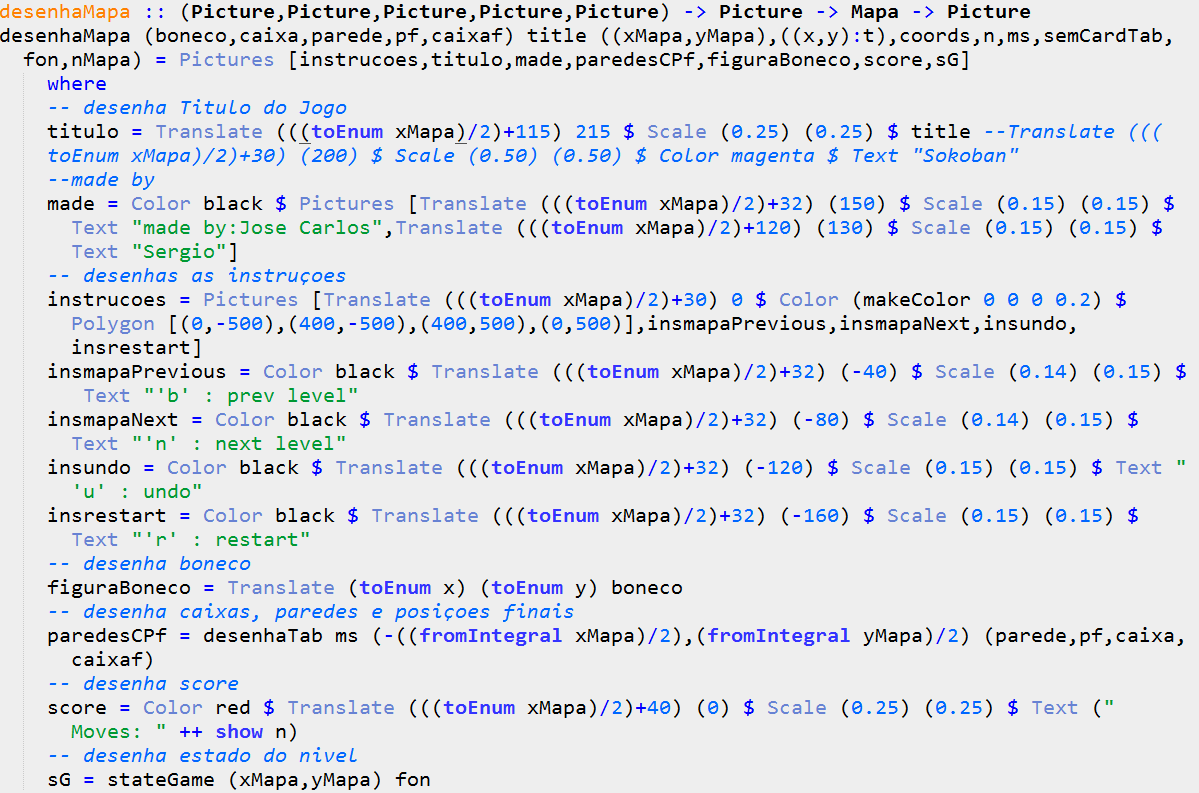
\includegraphics[height=9cm, width=15cm]{desenhamapa}
\end{figure}
  \item[reageF :] Reage ao "teclar" do jogador. Este jogo contém funcionalidades adicionais como o restart e o undo. Esta função recebe um evento do utilizador dado pelo teclado e um mapa(tipo) e perante determinado evento, age de acordo com o mesmo. Portanto, quando a tecla R é pressionada, é chamada a função auxiliar restart que reinicia o nível e, quando a tecla U é pressionada, é chamada a função auxiliar undo que volta um passo atrás no nível.
\begin{figure}[!htb]
\centering
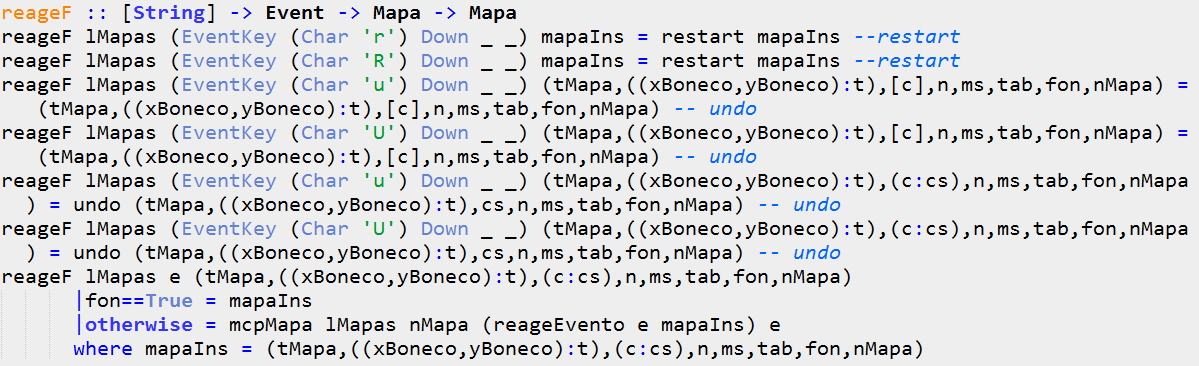
\includegraphics[height=5cm, width=15cm]{reageF}
\end{figure}
\newpage
  \item[reageEvento :] Reage ao pressionar das setas do teclado, movendo o boneco 40 pixels numa determinada direção. Esta é a função que origina o movimento no jogo e recebe um evento do teclado do utilizador e um mapa(tipo) e devolve outro mapa(tipo). Como base há o uso da auxiliar moveBoneco que mexe as coordenadas x e/ou y do boneco conforme a tecla pressionada. No entanto, há algumas condições a ter em conta relativamente ao movimento da personagem já que se no movimento encontrar parede, então não move; se encontrar uma caixa verifica se a caixa pode ser mexida. Se sim, então a caixa e o boneco mexem-se. Se não, então não há movimento.
  \begin{figure}[!htb]
\centering
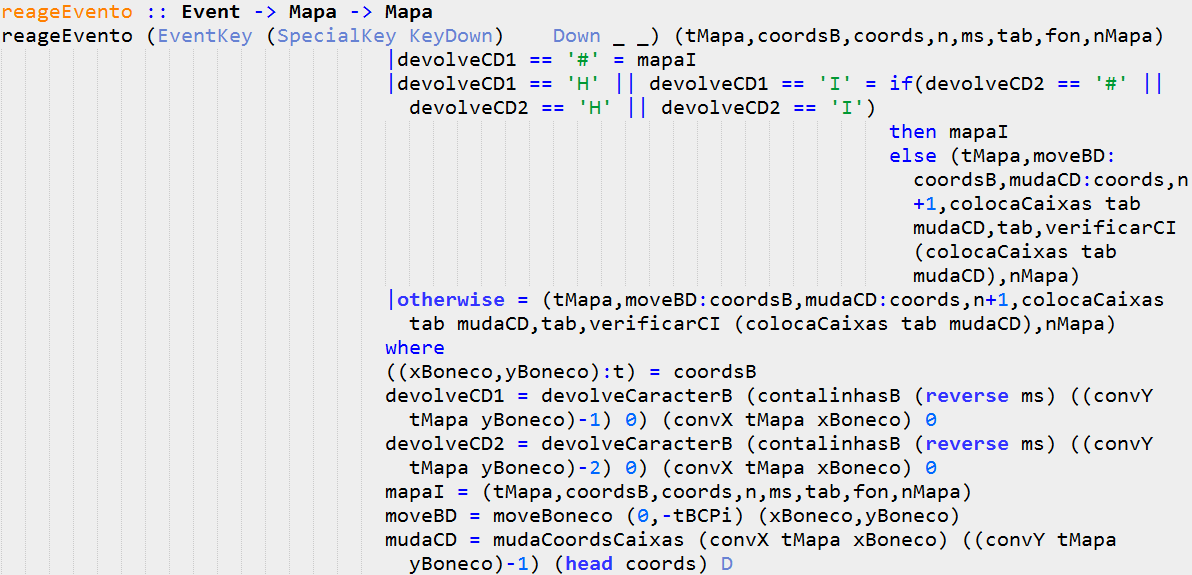
\includegraphics[height=7cm, width=15cm]{reageEvento}
\end{figure}
\end{description}

Funções adicionais que acrescentam originalidade e variedade ao jogo:
\begin{description}
  \item[restart :] Reinicia o nível;
  \item[undo :] Volta um passo atrás;
  \item[mcpMapa :] Permite passar para o nível anterior ou seguinte.
\end{description}

\pagebreak
\subsection{Testes}
Para a realização da tarefa D, criámos testes que nos pudessem dar outputs diferentes para, assim, podermos atestar à fiabilidade do código. Alguns dos testes:

\begin{multicols}{4}
\begin{verbatim}
TESTE 1
###################
#####   ###########
#####   ###########
#####   ###########
###      ##########
### # ## ##########
#   # ## #####  ..#
#               ..#
##### ### # ##  ..#
#####     #########
###################
11 2
5 8
7 7
5 6
7 6
2 3
5 3
ULDRUU
INCOMPLETO 3 
\end{verbatim}

\columnbreak

\begin{verbatim}
TESTE 2
###################
#####   ###########
#####   ###########
#####   ###########
###      ##########
### # ## ##########
#   # ## #####  ..#
#               ..#
##### ### # ##  ..#
#####     #########
###################
11 2
2 16
ULDRUU
FIM 0
\end{verbatim}

\columnbreak

\begin{verbatim}
TESTE 3
########
##    .#
########
2 1
3 1
ULDRUURR
FIM 3
\end{verbatim}
\columnbreak

\begin{verbatim}
TESTE 4
########
##    .#
########
2 1
3 1
ULDRUURRRULD
FIM 3
\end{verbatim}
\columnbreak
\end{multicols}

Para a realização da tarefa E, criámos testes que nos pudessem também dar outputs diferentes para, assim, podermos atestar à fiabilidade do código. Estes testes estão presentes no próprio código da tarefa (ficheiro: TarefaE.hs). De seguida, mostraremos alguns dos testes:

\begin{spverbatim}
test3 = TestCase (assertEqual "for Circle 20," "40 40" (fTeste (Circle 20)))
test8 = TestCase (assertEqual "for Color white (Circle 20)," "40 40" (fTeste (Color white (Circle 20))))
test9 = TestCase (assertEqual "for Rotate 57 (Circle 20)," "40 40" (fTeste (Rotate 57 (Circle 20))))
test12 = TestCase (assertEqual "for Pictures []," "0 0" (fTeste (Pictures [])))
\end{spverbatim}
\pagebreak

\subsection{Resultado Final}
\begin{figure}[!htb]
\centering
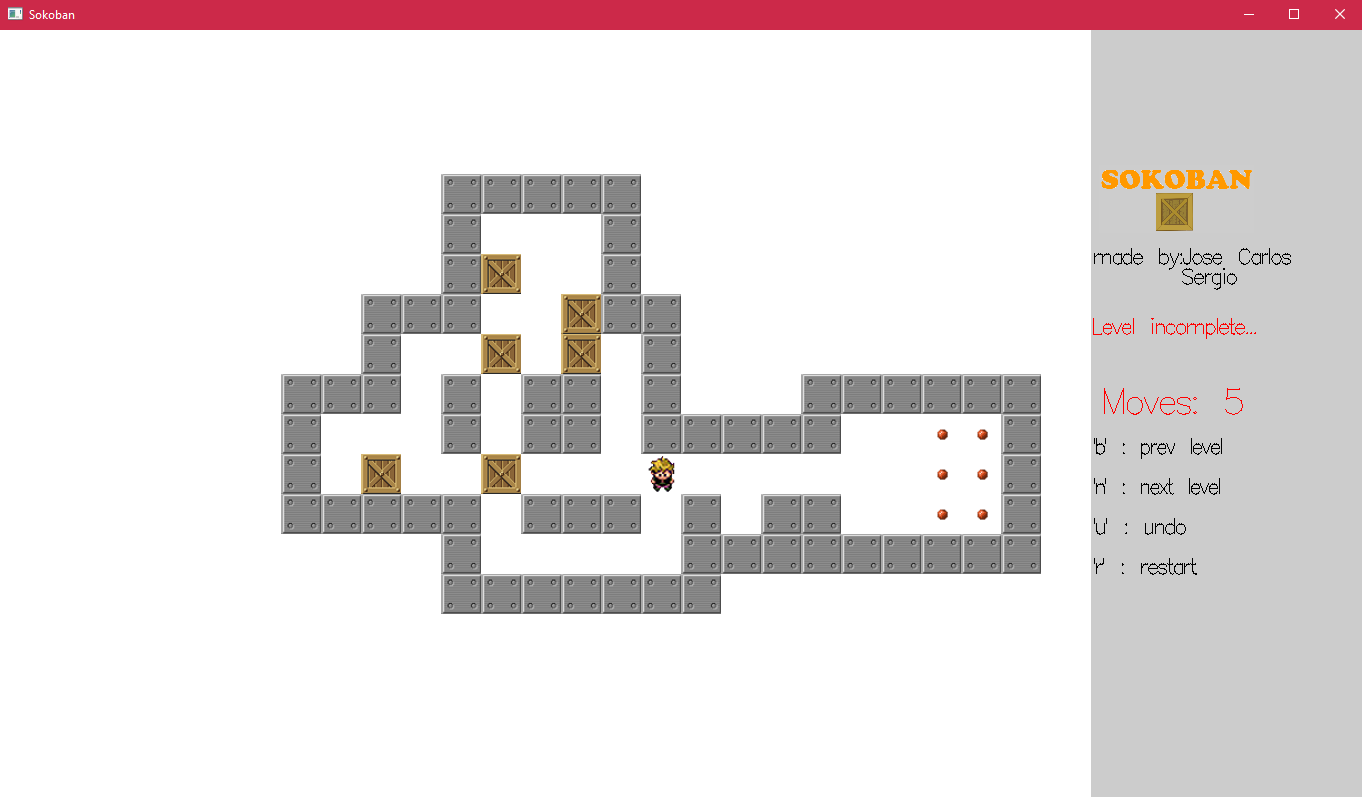
\includegraphics[height=10cm, width=15cm]{jogofinal}
\end{figure}


\section{Conclusões}
\label{sec:conclusao}
Este projeto de duas fases serviu para aprofundarmos o conhecimento da linguagem Haskell, assim como as bibliotecas que lhe estão associadas. Achámos que, com a realização de um trabalho deste tipo permite uma consolidação proveitosa da linguagem, não só em termos teóricos como também em termos práticos e acaba por ser uma forma diferente de cimentar os conteúdos de Programação Funcional. Permite também melhorar as habilidades na resolução de problemas. Concluímos também que:

\begin{itemize} 

        \item É possível fazermos coisas engraçadas e aplicarmos com grande utilidade aquilo que à partida e, numa primeira fase, nos parece demasiado limitado, isto no que diz respeito à linguagem Haskell; 
        \item Podemos ficar com uma ideia do que é programar e trabalhar em equipa, e neste contexto, ressalta-se a importância e a utilidade que encontramos no "svn"; 
        \item Permite desenvolver capacidades no que toca à produção de relatórios em Latex.
\end{itemize}

\end{document}